\documentclass{article} 

\usepackage{graphicx}

\usepackage{amsmath,amsthm,amssymb}

\newtheorem{problem}{Problem} 

\theoremstyle{definition} 

\newtheorem*{solution}{Solution} 

\begin{document} \title{Assignment 2} 

\author{Weishi Wang, ID 260540022} 

\date{\today}

\maketitle

\begin{problem} 
\textbf{Negation of predicates.} For each of the sentences below,\\
	i. write it using symbolic logic notation, using the indicated predicates;\\
	ii. find the negation of your sentence from (i) and simplify as much as possible; and\\
	iii. re-write your answer from (ii) in English ( with appropriate mathematical notation where applicable). Your answer should match the one from (ii) exactly; answers which differ will not receive full marks, even if logically equivalent.\\\\
(a) Something is rotten in the state of Denmark. [D(x): x is in Denmark; R(x): x is rotten]\\
(b) For every real number \(\varepsilon\) \(>\) 0 there is a positive real number N such that x \(>\) N implies that \(| f(x)\) - L\(|\) \(<\) \(\varepsilon\). [B(x,y): x \(>\) y]\\\\


\end{problem}


\begin {solution}
(a)\\
i.	\(\exists\) x (D(x) \(\wedge\) R(x))\\\\
ii.	Negation: \\
\(\neg\)[\(\exists\)x (D(x) \(\wedge\) R(x)]\\
\(\forall\)x \(\neg\)[(D(x) \(\wedge\) R(x)]\\
\(\forall\)x (\(\neg\)D(x) \(\vee\) \(\neg\)R(x))\\\\
iii.	Everything is either not rotten or not in the state of Denmark.\\\\
(b)\\
i.	The domain is \(\mathbb{R}\)\\
\(\forall\)\(\varepsilon\) \(> 0\) \(\exists\)N \(> 0\) \(\forall\)x [B(x,N) \(\Rightarrow\) (\(|f(x) - L| <\)\(\varepsilon\))]\\\\
ii. Negation:\\
\(\neg\)[\(\forall\)\(\varepsilon\) \(> 0\) \(\exists\)N \(> 0\) \(\forall\)x (B(x,N) \(\Rightarrow\) (\(|f(x) - L| <\)\(\varepsilon\)))]\\
\(\exists\) \(\varepsilon > 0\) \(\forall N > 0\) \(\exists\)x \(\neg\)[B(x,N) \(\Rightarrow\) \(|f(x) - L| <\)\(\varepsilon\)]\\
\(\exists\) \(\varepsilon > 0\) \(\forall N > 0\) \(\exists\)x \(\neg\)[\(\neg\)B(x,N) \(\vee\) \(|f(x) - L| <\)\(\varepsilon\)]\\
\(\exists\) \(\varepsilon > 0\) \(\forall N > 0\) \(\exists\)x [B(x,N) \(\wedge\) \(\neg\)(\(|f(x) - L| <\)\(\varepsilon\))]\\
\(\exists\) \(\varepsilon > 0\) \(\forall N > 0\) \(\exists\)x [B(x,N) \(\wedge\) (\(|f(x) - L|\) \(\geq\) \(\varepsilon\))]\\\\
iii. There is a positive real number \(\varepsilon\) such that for all positive real number N, there exists a real number x greater than N and satisfies \(|f(x) - L|\) \(\geq\) \(\varepsilon\).\\\\


\end {solution}

\begin{problem}
\textbf{Rules of inference.}

(a) Verify the transitivity inference rule by using a truth table (do not just give the table, but also clearly state why your table shows the argument is valid).\\

(b) Verify the modus tollens inference rule by showing an appropriate statement that is a tautology using only logical identities.\\

(c) Use the rules of inference given on the handout to determine if the following argument is valid. Clearly state which rules you are using (youmay symbolize if it is helpful).\\

	If I study, the I will pass.
	
	If I do not go to a movie, then I will study.
	
	I did not pass.\\
	\noindent\rule{8cm}{0.4pt}
	
	Therefore, I went to a movie.\\\\

\end{problem}

\begin{solution}

(a) The transitivity states that if P \(\Rightarrow\) Q and Q \(\Rightarrow\) R, then P \(\Rightarrow\) R. Thus, we need to prove that [(P \(\Rightarrow\) Q) \(\wedge\) (Q \(\Rightarrow\) R)] \(\Rightarrow\) (P \(\Rightarrow\) R)

\begin{displaymath}
\begin{array}{ c|c|c|c|c|c|c|c }
% |c c|c| means that there are three columns in the table and
% a vertical bar '|' will be printed on the left and right borders,
% and between the second and the third columns.
% The letter 'c' means the value will be centered within the column,
% letter 'l', left-aligned, and 'r', right-aligned.
P & Q & R & P \Rightarrow Q & Q \Rightarrow R & P \Rightarrow R &  (P \Rightarrow Q) \wedge (Q \Rightarrow R) &  [(P \Rightarrow Q) \wedge (Q \Rightarrow R)] \Rightarrow (P \Rightarrow R)  \\ % Use & to separate the columns[
\hline % Put a horizontal line between the table header and the rest.
T & T & T & T & T & T & T & T\\
T & T & F & T & F & F & F & T\\
T & F & T & F & T & T & F & T\\
T & F & F & F & T & F & F & T\\
F & T & T & T & T & T & T & T\\
F & T & F & T & F & T & F & T\\
F & F & T & T & T & T & T & T\\
F & F & F & T & T & T & T & T\\
\end{array}
\end{displaymath}
According to the truth table, we notice that [(P \(\Rightarrow\) Q) \(\wedge\) (Q \(\Rightarrow\) R)] \(\Rightarrow\) (P \(\Rightarrow\) R) is a tautology. This proves the transitivity.\\\\
(b) modus tollens states:

	P \(\Rightarrow\) Q
	
	\(\neg\)Q
	
	\noindent\rule{2cm}{0.4pt}
	
	\(\therefore\) \(\neg\)P\\
	
	
	This means that If P \(\Rightarrow\) Q is true, and \(\neg\) Q is true, then \(\neg\) P must be true. Let's try to prove this:
	
	(P \(\Rightarrow\) Q) \(\equiv\) (\(\neg\)P \(\vee\) Q) (Conditional)
	
	(P \(\Rightarrow\) Q)	\(\equiv\) \(\neg\)(P \(\wedge\) \(\neg\)Q) (Reverse DeMorgan's laws)
	
	The statement states that P \(\Rightarrow\) Q is true, and \(\neg\)Q is true as well, therefore:
	
	\(\mathbb{T}\) \(\equiv\) \(\neg\)(P \(\wedge\) \(\mathbb{T}\))
	
	\(\mathbb{T}\) \(\equiv\) \(\neg\)P (Identity)\\
	
	Thus, \(\neg\) P is true. This proves that if P \(\Rightarrow\) Q is true, and \(\neg\) Q is true, then \(\neg\) P is true. Therefore, modus tollens is verified.\\\\


\end{solution}

\begin{problem}
\textbf{Set operations.} Let A = \{ n \(\in\) \(\mathbb{N}\) \(|\) n \(>\) \(7\) \}, 

B = \{q \(\in\) \(\mathbb{Q}\) \(|\) \(|q-2|\) \(<\) 1\}, C = \{r \(\in\) \(\mathbb{R}\) \(| {r}^3 - r = 0\)\} and D = \{1, 2, \{1,2\}\}. Find each of the following (reall that P(X) denotes the power set of X). Do not use "..." in your answer; give clear rules for set membership if you need them.

(a) A \(\oplus\) C \: (c) C \(\cup\) D \: (e) B \(\setminus\) (A \(\oplus\) C) \: (g) (A \(\setminus\)B) \(\setminus\) (C \(\setminus\)\(\overline{\rm D}\))

(b) A \(\cap\) D \: (d) \{1,\{2\}\} \(\cup\) D \: (f) \{\o\} \(\setminus\) P(A) \: (h) P(D) \(\cap\) D\\\\

\end{problem}

\begin{solution}

(a) A \(\oplus\) C = \{-1, 0, 2, 3, 4, 5, 6\}\\

(b) A \(\cap\) D = \{1, 2\}\\

(c)  C \(\cup\) D = \{-1, 0, 1, 2, \{1, 2\}\}\\

(d) \{1,\{2\}\} \(\cup\) D = \{1, 2, \{2\}, \{1, 2\}\}\\

(e) B \(\setminus\) (A \(\oplus\) C) = \{q \(\in\) \(\mathbb{Q}\) \(|\) (1 \(<\) q \(<\) 2) \(\vee\) (2 \(<\) q \(<\) 3) \}\\

(f)  \{\o\} \(\setminus\) P(A) = \o\\

(g) (A \(\setminus\)B) \(\setminus\) (C \(\setminus\)\(\overline{\rm D}\)) = \{1, 3, 4, 5, 6\}\(\setminus\)\{1\} = \{3, 4, 5, 6\}\\

(h) P(D) \(\cap\) D = \{\{1\}, \{2\}, \{1, 2\}, \{\{1, 2\}\}, \{1, \{1, 2\}\}, \{2, \{1, 2\}\},

\{1, 2, \{1, 2\}\}, \o\} \(\cap\) \{1, 2, \{1, 2\}\} = \{\{1, 2\}\}\\\\

\end{solution}


\begin{problem}
\textbf{Venn diagrams.} Draw a Venn diagram for each of the following.\\

(a) A \(\cap\) \(\overline{B \cup C}\) \: (b) \(\overline{A} \setminus (B \cup \overline{C}\)) \: (c) \(( A \cup B) \oplus ( C \setminus B\))\\\\

\end{problem}

\begin{solution}
\begin{figure}
\centering
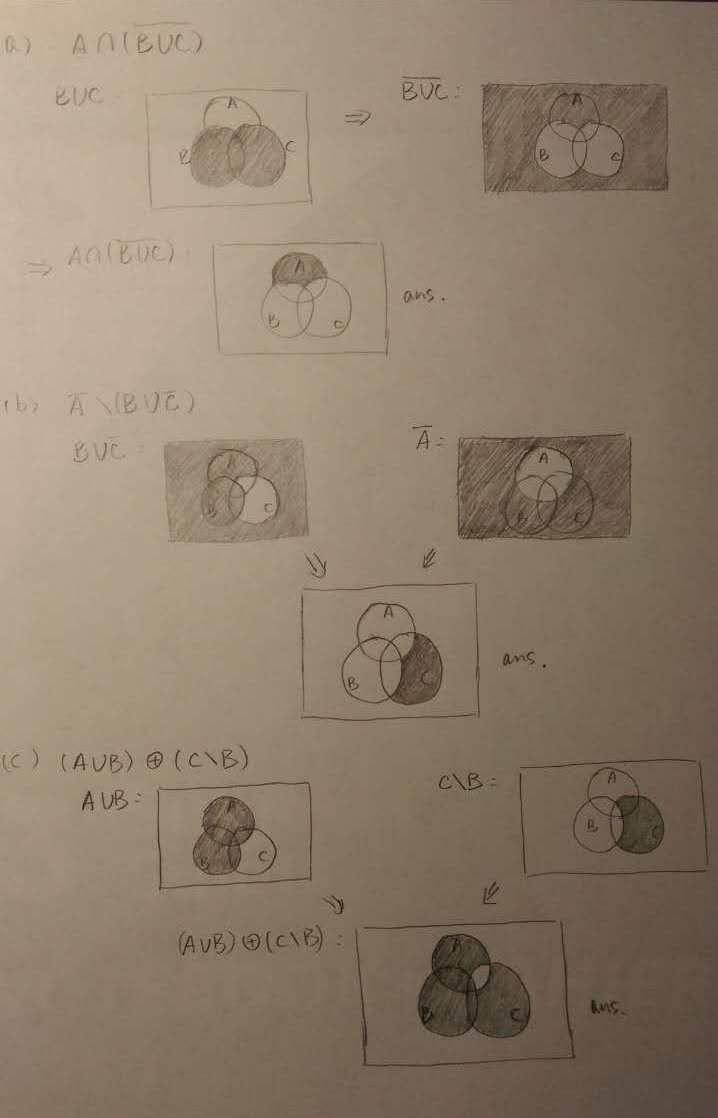
\includegraphics[width=1.1\textwidth] {Q4.jpeg}
\end{figure}
\end{solution}


\end{document}